\chapter{Presentation of Results}
\section{Introduction}
The sections and subsections in this chapter describe the implementation, testing and results of the project. It starts by discussing how the web application to handle students' results was built. It then describes how The decentralised file storage element of the system was put up and how all these elements were integrated together.

\section{System Implementation}
This section and the subsections beneath it describe the Implementation and results of the project. Different elements of the system were built using different tools. The subsections below further describe how each element was built to get the complete system running from the web application that handles the students' results to the decentralised storage of transcripts and blockchain store for the hash values.

\subsection{Results System}
The results system is an element of the system where results are initially entered and processed before they are finally stored on a decentralised network. This system is built to be accessed by students, administrative assistants, the academic registrar and the system administrator. All these have different levels of priviledges when accessing the system for example, a student is only able to view his results and not edit them. \\~\\
The first attempt to build this system was done entirely on a blockchain network using smart contracts. A smart contract in simple terms can be defined as computer code running on top of a blockchain that controls transfer of digital currencies or assets between parties under certain conditions\cite{20}. This approach was not feasible and economically sound because alot of writes would have to be done to the blockchain and this costs ether. Ether is fuel used on the ethereum blockchain network. The latter attempt involved building a web based centralised application that handles the results which are later stored in a decentralised manner. Building this application was broken down into the following parts.

\subsubsection{Front End}
The front end of the application runs on a web browser like google chrome or mozilla firefox. These web browsers have a uniform support for various programming languages that are used together to build the web pages we know today. Described below are the programming languages used to build the front end of the results system.\\\\
\textbf{HTML(Hyper Text Mark-up Language):} HTML is the standard markup language for creating web pages applications. Using HTML elements as the building blocks these pages, we were able to insert images, interactive forms among other items on the HTML pages.\\\\
DDDDDDDDDDDDDDDDDDDDDDform code snippetWDDDDDDDDDDDDDDD
DDDDDDDDDDDDDDDDDDDDDDForm outputDDDDDDDDDDDDDDDDDDDDDD
During the development process, the web browser received the the HTML documents from local storage.\\~\\
\textbf{CSS(Cascading Styles Sheet): }This is a style sheet language used to describe the presentation of a document written in a markup language like HTML in the case of this project. Some of the styling used on the web pages were fetched from CSS files in the bootstrap packages. \\\\
CSS was used to add animations to the web pages, style and position different elements in the HTML pages. External CSS was used in the development of the results system. External CSS as opposed to internal CSS, has the styling of the web page done in another file and that file just refereed to by the HTML web pages. This availed the same styling to be applied to multiple HTML files.\\~\\
QQQQQQQQQQQQQQreference snippetQQQQQQQQQQQQQQQQQ\\~\\
\textbf{JavaScript: }JavaScript is a light weight interpreted programming language. For the domain of this project, JavaScript was majorly used to make the web pages interactive and dynamic. JavaScript used in the construction of the results system was used to give alerts when a user logs in.\\~\\
There are already existing open sourced web development tools that support the development of web pages. These tools were chosen majorly because they support the programming languages described earlier. Explained below is how these tools were used to achieve the front end of the results system.\\~\\
\textbf{Visual Studio Code: }This is a light weight text editor that runs remotely on a desktop. VS code  used to write code for most parts of the implementation. VS code was installed on local computers of various team members and each configured with a github account to ease the collaboration process. The configuration was done on a command line interface known as the terminal. All the changes pushed to github were done using commands and so were the changes pulled from github.\\\\
\textbf{Twitter bootstrap: }This is an open-source HTML, CSS and JavaScript framework that is used in front-end web development. We used this to enhance the appearance of the various pages of the application and also make them responsive. \\\\
\textbf{Github: }Github is a web based hosting service for version control using git, mostly used for computer code. We used this to co ordinate work among the various team members. Whenever a team member made changes, they were pushed to github and the other team members would pull the changes on their remote computers.\\~\\
\textbf{Browser Developer tools: }This is an inbuilt functionality in most web browsers that can be used to inspect the currently-loaded web page. It shows HTML elements, style of the web page and JavaScript file written for the page.

\subsection{Back end}
Up to this part of the project, the students results are still stored in a centralized manner on a server. During the development process, the server was run locally on a Desktop Computer. There are a number of open source local development environments that can be used to develop the back end of a web application for example WampServer, Laragon, XAMPP, among others. XAMPP was used for the case of this project.\\~\\
\textbf{XAMPP}\\~\\
XAMPP which stands for Cross-platform, Apache MariaDB, PHP and Perl is a lightweight application that enables developers create a local web server for testing purposes. XAMPP contains key components to set up a web server i.e. Apache server, MariaDB for the database and an interpreter for the scripting language PHP. Explained below in detail are the components of XAMPP and how they were used to achieve the target of the project.\\~\\
\textbf{PHP }\\PHP is a general purpose scripting language popularly used for web development with over 244 million sites that were using it by the year 2013. For the results system, PHP was majorly used to manipulate database values.\\~\\
PHP has a number of libraries that can be called to perform specific functions. One of the aims of this project is to ensure safe storage of students' transcripts. These transcripts are generated from the results system as a PDF which is later stored on a decentralized network as we'll later see in... PHP offers a number of libraries to generate PDFs for example FPDF, mPDF, DOMPDF among others. DOMPDF is the library chosen for this project.\\~\\
\textbf{MySQL: }SQL stands for Structured Queried Language. It is a database language used for database creation, deletion, fetching rows and modifying them. It is one of the components provided in the XAMPP package. MySQL also consists of functions that are available for use when writing PHP scripts. In this project, these functions were majorly used to manipulate values in the database.
\textbf{Apache Server: }Apache is an open-source free web server software powering around 46\% of web servers world wide. It is one of the components availed in the XAMPP package able to run locally. To access the web application locally, Apache is ran and the following url, http://127.0.0.1/ is used to access the server. Through out the development of the results system, Apache was run offline.
\subsection{IPFS integration}
IPFS is a protocol that establishes the peer-to-peer network with resources addressed based on their content instead of the physical location. Our system uses this protocol with aim of guaranteeing users a decentralized and unalterable storage at a fraction of the price they  would have to give in transaction fees.\\
The PDF file generated by the Results system implementation above is the input of this next phase of imlementation.\\
We implement this protocol in such a way that the network is not going to store files once you add them. Adding files to IPFS does not upload them anywhere and only means that you add them to the local repository you host on your node. Therefore, what our system does is we create a hashed representation of the file and share this as a reference to the file.\\\\
XXXXXXXXXXXXXXXXXXXXXXXXXXXXXXXXXXXXXXXXXXXXXXXXXXXXXXXXXXXXXXXXXXXXXXXXXXXXXXXXXXXXXXXXXXXXXXXXXXXXXXXXXXX
\\\\
However, during the implementation of this project, we realized that connecting to the Ethereum blockchain is messy and complicated. We faced challenges which include:
\begin{enumerate}
\item The expense of storing data on the Ethereum blockchain
\item Complexity in configuring the Ethereum geth client and
\item Scalability of infrastructure would be tough
\end{enumerate}
\subsubsection{Infura}
In attempt to overcomethe challenges listed above, we used Infura. Infura is a set of tools used to create an application that connects to the Ethereum blockchain. It interacts with the Ethereum blockchain and runs nodes on behalf of our system.\\\\
Using Infura's API made our system fast, scalable and provides extra data storage. However, despite the fact that Infura offers to do that work for us, it brings with it the cost of increased centralization.
The output of this subsystem is a hashed  URL which is a reference to our PDF file.

\subsection{Ethereum blockchain}
As mentioned in the above section, using Infura and IPFS provides extra data storage for us. This is done is such a way that instead of storing the entire file on-chain, data can be stored separately i.e locally on a server from the results system in section 5.2.1, with just a hash stored on the blockchain.\\By storing the hash on the Ethereum blockchain,the system takes advantage of the blockchain principles of Immutability, Disintermediation and Transparency.
STILL WORK IN PROGRESS HERE
XXXXXXXXXXXXXXXXXXXXXXXXXXXXXXXXXXXXXXXXXXXXXXXXXXXXXXXXXXXXXXXXXXXXXXXXXXXXXXXXXXXXXXXXXXXXXXXXX
\begin{figure}[!h]
\center
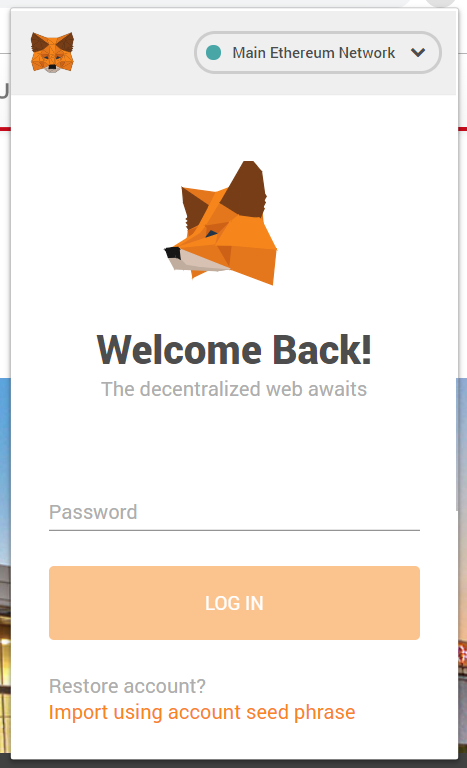
\includegraphics[scale=0.6]{images/metamasklogin.png}
\caption{Loging into the ethereum network}
\end{figure}

\subsubsection{Results}
\textbf{Viewing Results}\\~\\
This page can be accessed by a logged in student or an administrative assistant. The student can only view his/her results whereas the administrative assistant can view the results of various students.
\textbf{Manipulating results}\\~\\
In addtion to viewing results of various students, the adminsstrative assistant can also add/edit students’ results.
